%
% Chapter 9
%
\chapter{Amplifier Revision Design}
The investigation of the first generation amp design and testing gave the team useful insight into what needed to change for the next hardware revision. An evaluation of the goals of Nessie2 provided the basis for the redesign. By exploring a number of hardware architecture choices we begin to rebuild the amplifier circuit from the beginning.
\section{Nessie2 Overview}
As capabilities of the CSEs and SLEDS arrays have increased, so too have requests from customers. What started as a project to drive a single 512x512 LED array has turned into a deep investigation to the physics and hardware constraints involved with increasing frame rates and resolutions. The eventual goal is a system able to drive a 2Kx2K array at 2kHz \cite{chris}.\par To move toward this new goal a distributed architecture using smaller CSEs was envisioned. Each CSE would be capable of driving twice as many analog channels on a quadrant of the new 2Kx2K array. The array would therefore be driven by four synchronized systems. To accomplish synchronization and analog integrity at this scale required a complete remodeling of the system firmware and hardware architecture. A prototype "Multi-CSE" system has been constructed as a proof-of-concept. In short, this system broke the Dewar pins out to routing boards that accepted all four cable outputs from a CSE each. Using the full bandwidth of a system greatly increased potential resolution and frame rate such that no system was driving more than a normal SLEDS array's worth of pixels. More details on the Multi-CSE prototype and Nessie2 architecture can be found in Christopher Jackson's doctoral dissertation \cite{chris}. The biggest change directly relevant to the analog design was that the main system would only output unamplified DAC signals along new coaxial cables to the Dewar. The Dewar's main input board will contain cable receptacles and signal paths to mimic the old interface board. Included in this main input board will reside the new amplifiers. Moving this processing stage outside the system allowed us to consider many more functions for the amplifiers due to their proximity to the RIIC, which will be explored below.
\FloatBarrier
\begin{figure}[!htb]
	\centering
	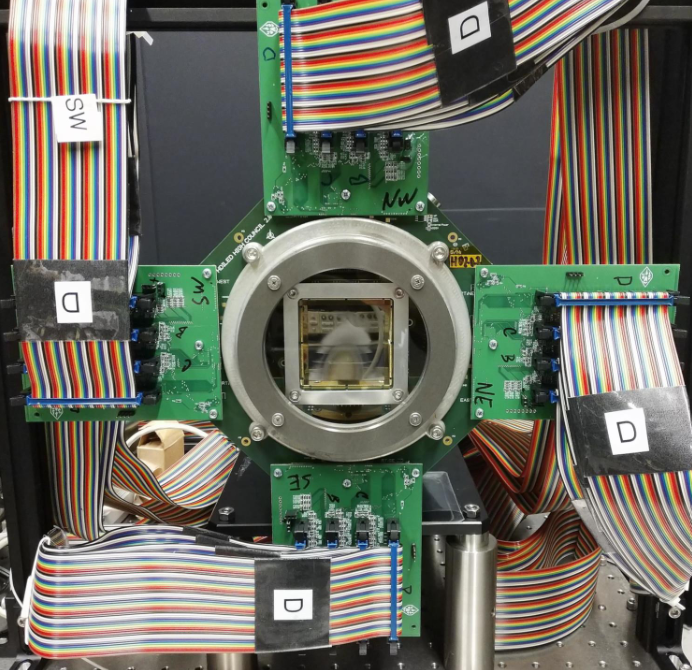
\includegraphics[]{multi_cse}
	\caption{Multi-CSE Prototype System \cite{chris}}
\end{figure}

\begin{figure}[!htb]
	\centering
	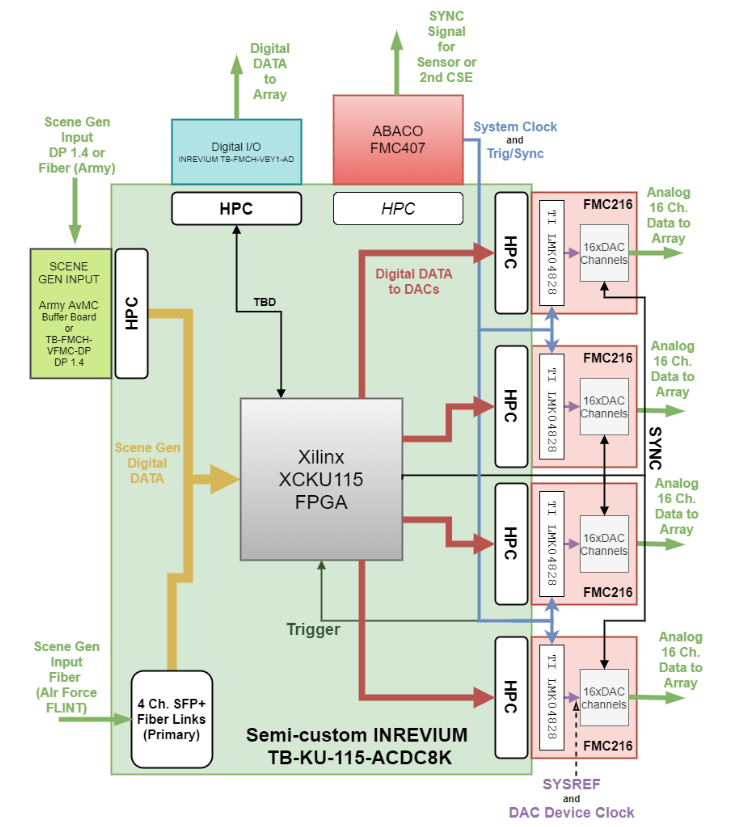
\includegraphics[]{nessie2_arch}
	\caption{Nessie2 System Architecture. Of note are the external ports for pre-amplified DAC output \cite{chris}.}
\end{figure}

\FloatBarrier

\section{Objectives}
The goal of the new amplifiers is twofold. The new system hardware already requires new amplifier cards as the current ones are too big. The hardware is due for a revision thanks to the excess of unpopulated components, empty connectors and unexplained design choices that waste space and money on the PCB. Additionally, due to the new increased resolution and frame rate, the system will have to be able to monitor and tune the amplifiers in order to maintain consistent output. These cards have to have some level of analog analysis and response to appropriately self-tune in conjunction with providing signals of the same (hopefully better) quality as the first generation. The self-tuning process is a response to the useless gain and offset potentiometers on the current design that do not affect gain or offset in any meaningful way. This is similar to the corrective role of the PC in creating NUC tables, but is system-level and intended to compensate for electrical differences in the large number of channels. An abstract architecture is as follows:
\begin{figure}[!htb]
	\centering
	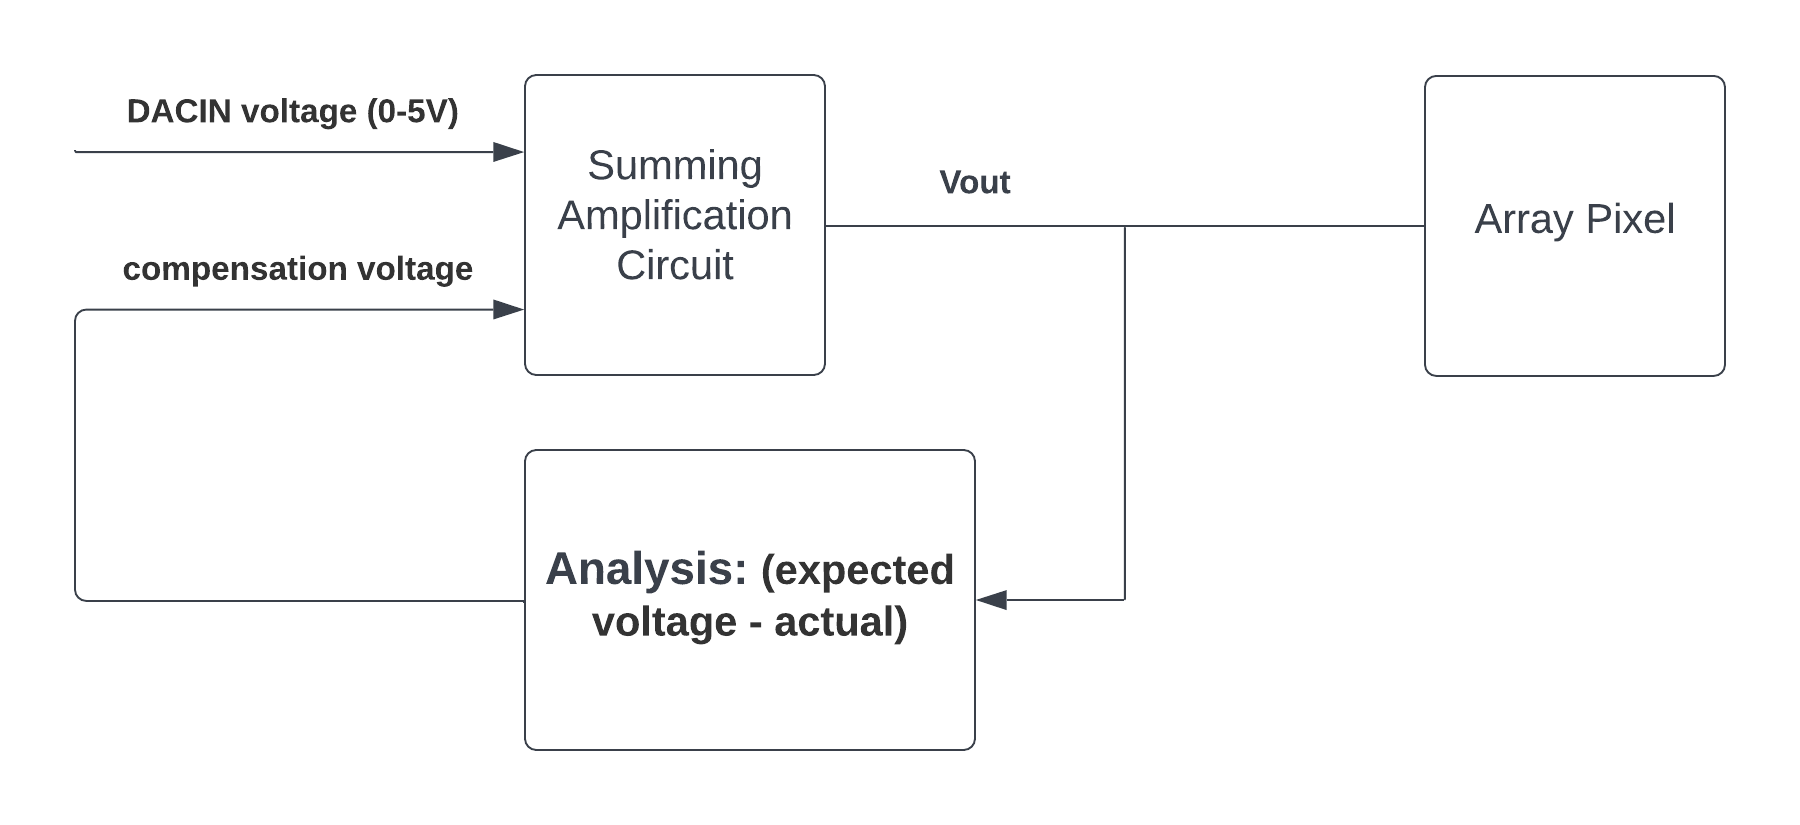
\includegraphics[]{amp2_block}
	\caption{Overview of the new analog component}
\end{figure}
\section{Amplifier Design Choices}
To properly analyze and respond to input, the system had to have some sort of analog probe point to read amplifier output. The simplest solution is to use an ADC to convert the reading into digital data. Once the voltage reading has been converted, a microcontroller or other appropriately small digital component should be able to read and react to this input. The result of the calculation can then be directly output as a voltage through a DAC, where the microcontroller will tell the DAC how much extra voltage to add to the summing amplifier component. By implementing a small subsystem that can automatically perform this task we remove the need for manual gain/offset controls and further ensure reliability for the new system.\par
Working on the previous test setup gave me a foundation for understanding real-time measurements and analog output. Since each channel can be individually tuned regardless of the others, the best architecture should utilize some level of parallelism to work through all 64 channels as quickly as possible.\par
\subsection{Parallelized Architecture}
The new Nessie2 system will have 64 analog channels. This in itself creates an interesting problem for the analog designers, as all 64 channels must be accessible for reads to our data processing system. An initial design consisted of placing 32 ADCs on each side of the amplifier board and having the microcontroller probe them.  Many microcontrollers come with multiple ADCs built-in but are usually not able to read from all of them at once. In the interest of pure parallelism, discrete ADCs on every single line would be the most effective solution to the problem. If individual components are going to be placed on every line rather than switching through them with an extra multiplexing layer, an FPGA would be the most effective way to analyze and respond to ADC inputs. The FPGA could be split into as many cores as required (64 in this case) and programmed to self-tune all channels at once when given a start signal. As the main controller, the FPGA would simply have to know what the targeted pixel voltage is (based on the DACIN value) and compare it to the amplifier output. If the amplifier is struggling to meet the target, the FPGA would command its channel's DAC to output compensation voltage that would be added to the DAC input through a summing amplifier. A parallelized architecture would also make testing simpler as individual cores or channels could be examined for issues. \par
While this would be an effective strategy for parallelzing the workload, discrete ADCs are prohibitively expensive and unavailable for purchase from many vendors due to the chip shortages at the time of writing. The amplifier additionally has size constraints at the moment that prevent us from adding too many components to the board. Hardware-level parallelism is always a balancing act between speeding up the task and adding more and more hardware to the design. While we believe a fully parallel amplifier tuning architecture is the best eventual goal, testing and development will for now be confined to a smaller scale microcontroller setup.
\FloatBarrier
\begin{figure}[!htb]
	\centering
	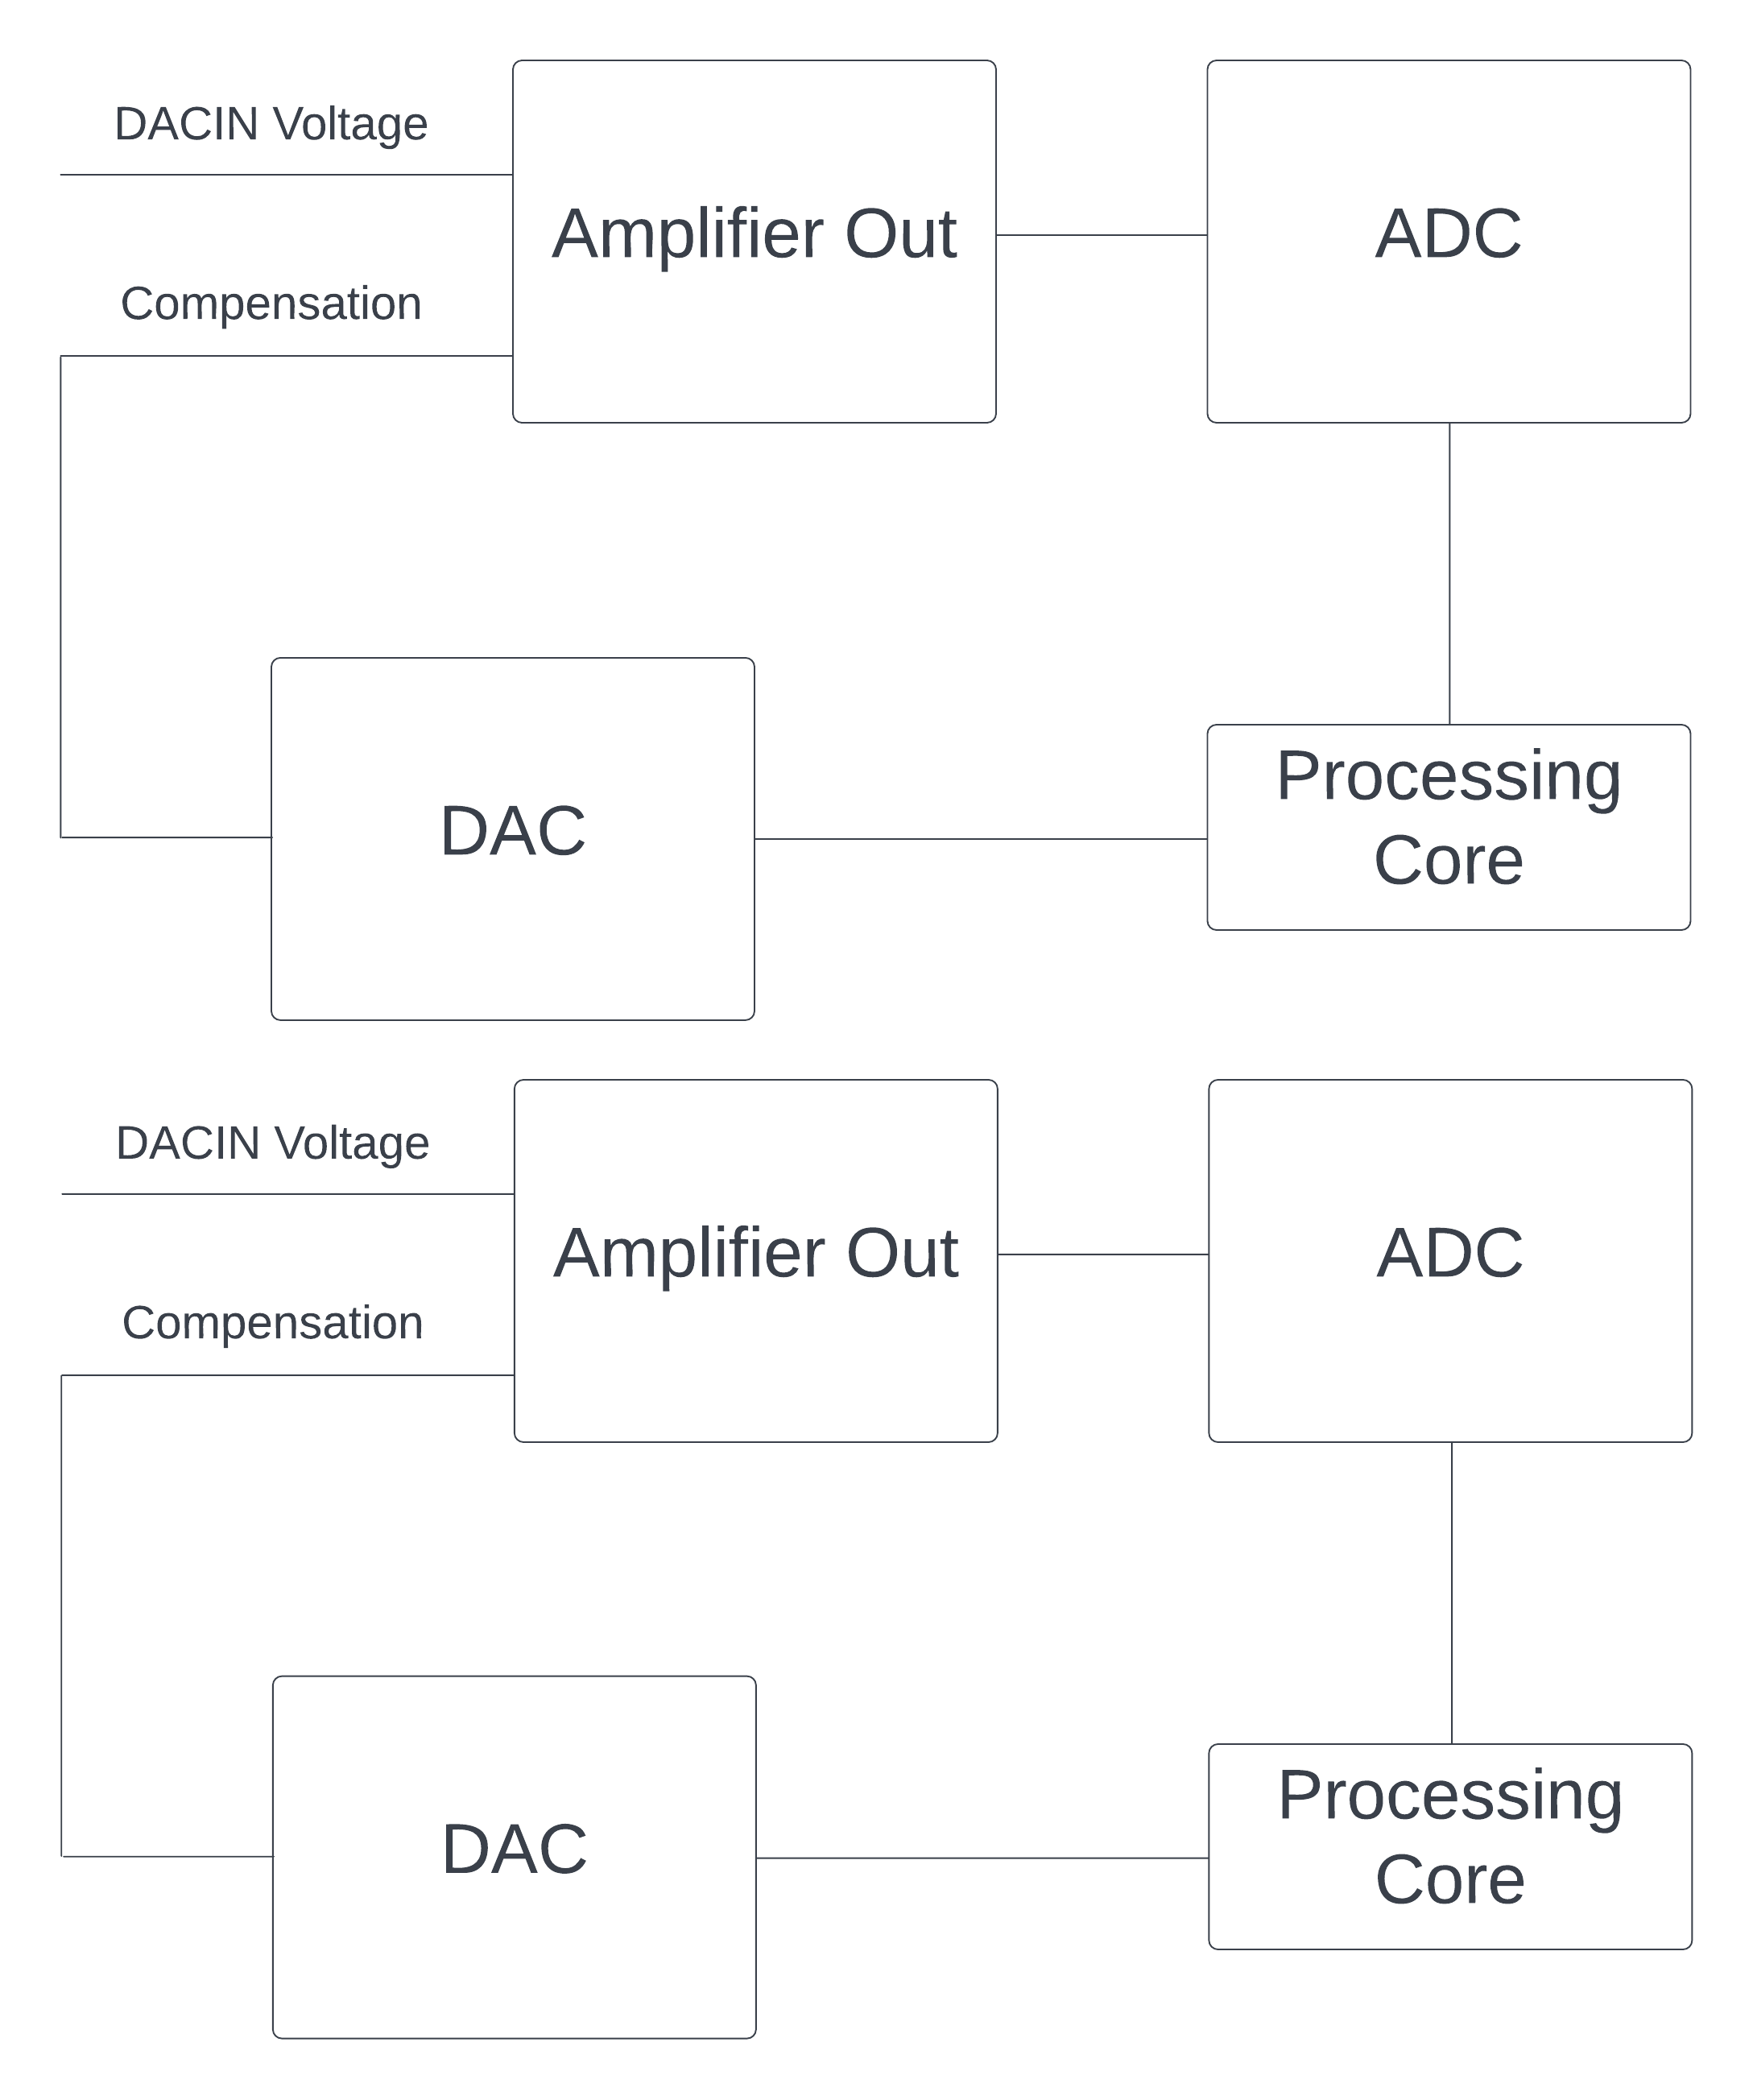
\includegraphics[width=0.5\textwidth]{fpga_amp_tuning}
	\caption{Block diagram of potential parallized architecture with 2 channels. Scalable to the physical limits of the FPGA.}
\end{figure}
\FloatBarrier
\subsection{Sequential Architecture}
To establish an effective parallel architecture in the future we must first solve the problem sequentially. To accomplish this a similar strategy will be taken of digitally analyzing input and outputting results to a DAC for summing. When performed sequentially, however, the large number of channels requires the designers to figure out an addressing or switching scheme to read from/write to all 64 channels. To accomplish this the channels can be grouped into multiplexing ICs which allow selection of a single input based on a select signal from a digital device. The main controller will be able to request a read from a specific channel which will activate select signals in a way that connects the selected channel to a single analog input. The main benefit of this approach is massively reduced cost and board size, as mux chips are small and the single ADC + DAC required are no longer an issue of cost. By testing this approach we plan to benchmark measurements and see if analysis can be carried out in a timely manner. Embedded solutions require clever programming and a full understanding of the hardware constraints.
\begin{figure}[!htb]
	\centering
	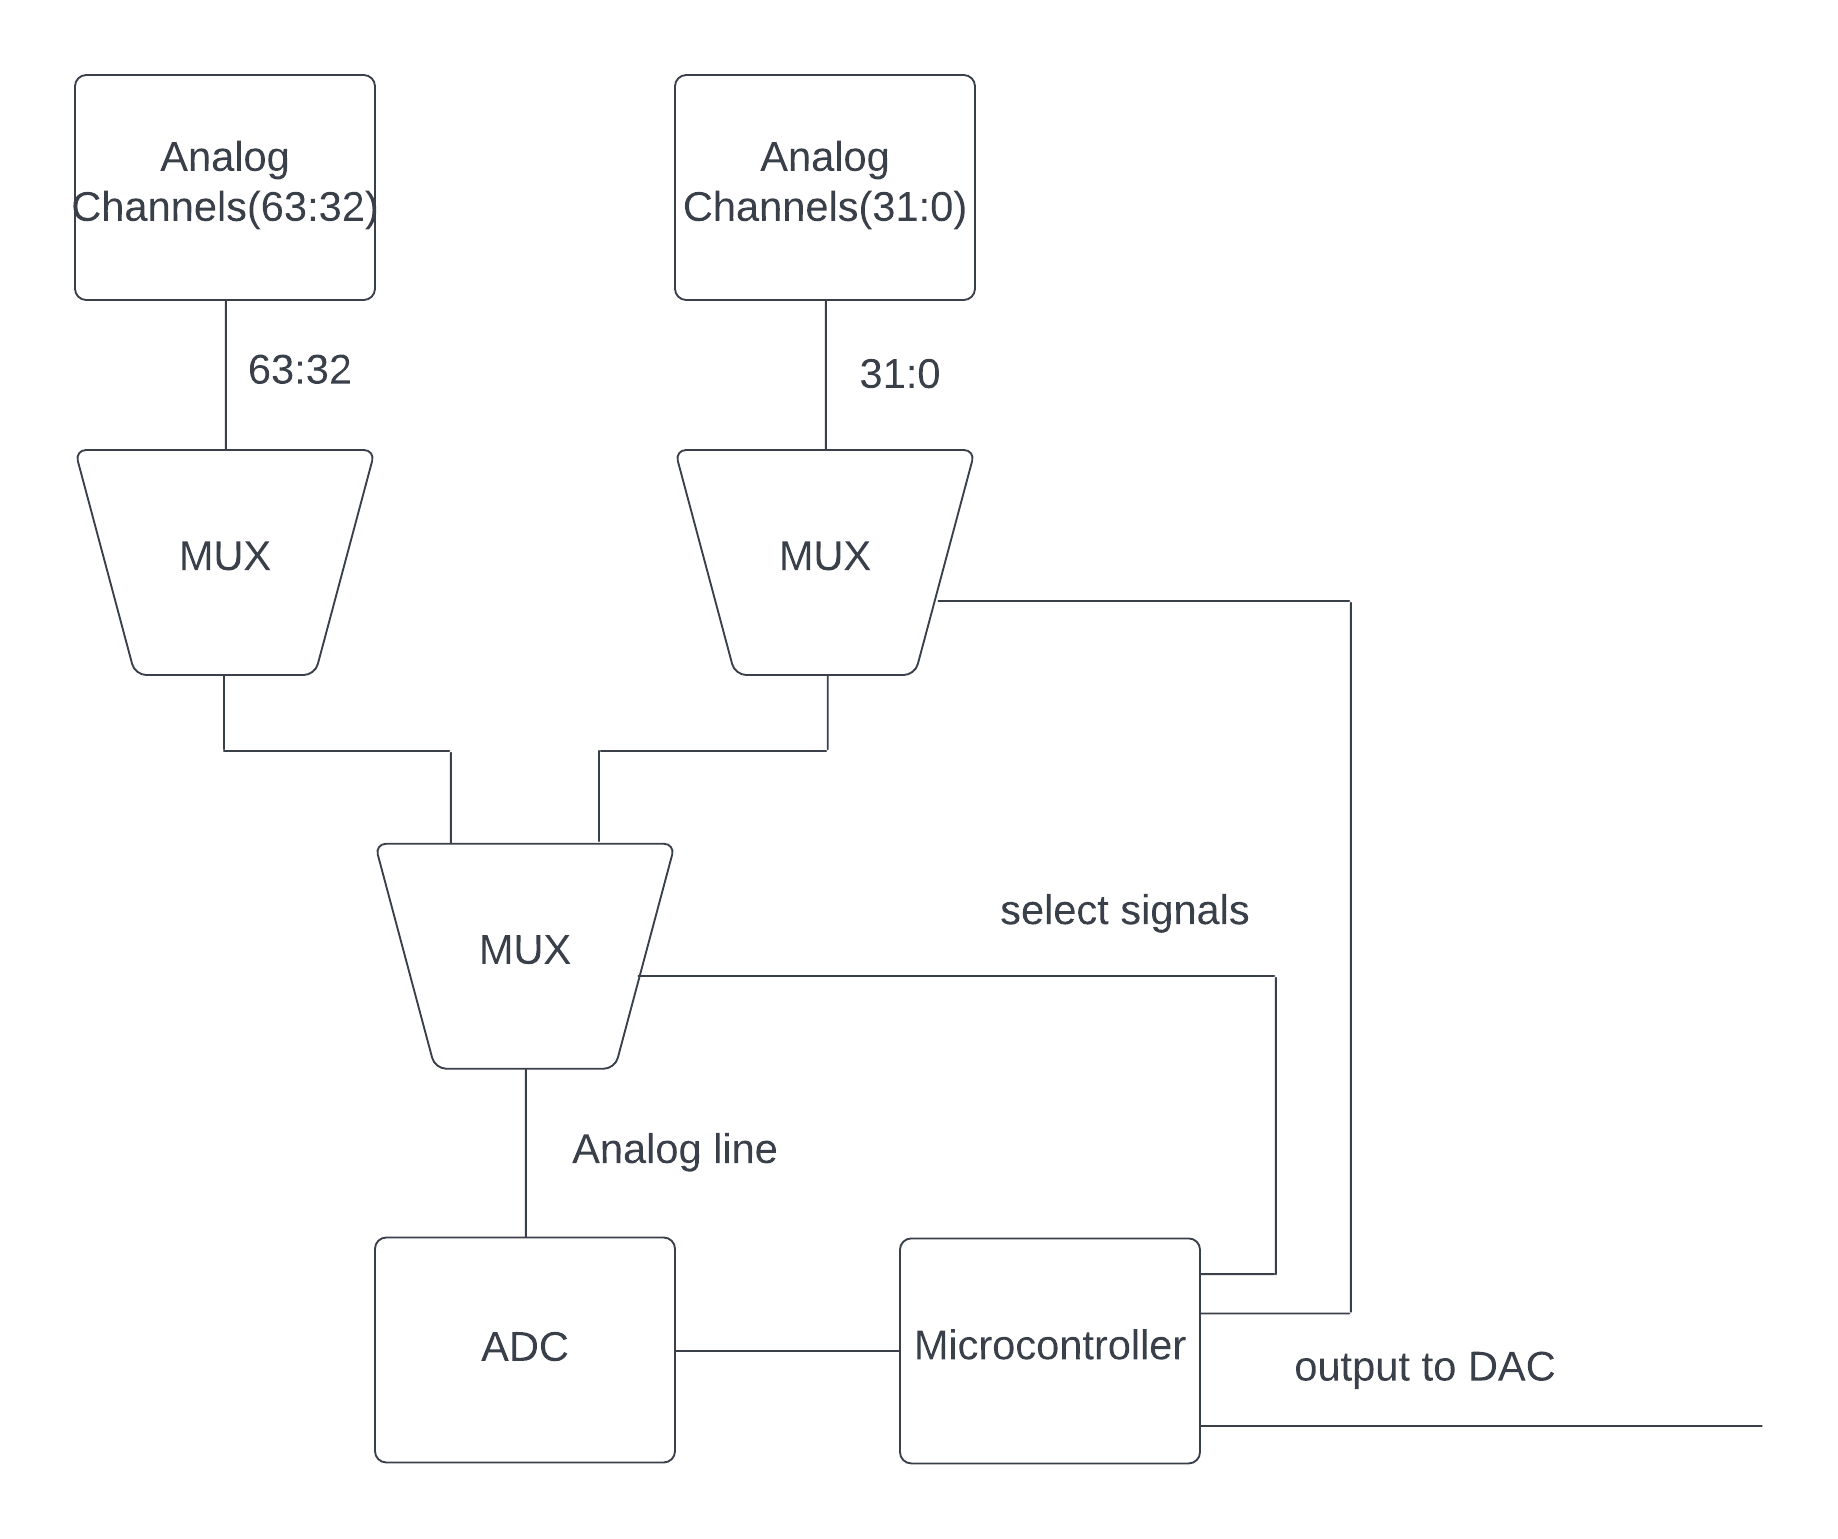
\includegraphics[width=\textwidth]{uc_amp_tuning}
	\caption{Microcontroller with multiplexed addressing}
\end{figure}